\chapter{Taint Analysis for Objects}
\label{field-tainting}

This chapter describes a concept for adding a sound taint analysis for member variables of objects to Pixy---the 2007 release of Pixy explicitly mentions this as a ``missing feature''.


\section{Modeling Objects and Member Variables}


\subsection{Class Declaration}

For the following code that declares a class with one field, the corresponding subtree of the PHP parse tree is depicted in figure~\ref{fig:parse-tree-foo-class} on page~\pageref{fig:parse-tree-foo-class}.

\begin{phpcode}
class Foo {
  var $field = 42;
}
\end{phpcode}

\paragraph{Note:} This piece of code still uses the PHP~4 way of declaring member variables. Using the PHP~5 way with access keywords\index{access keywords} like \texttt{public}, \texttt{protected} or \texttt{private} would work correspondingly.\index{public (keyword)}\index{protected (keyword)}\index{private (keyword)}

\begin{figure}[htb]
  \begin{center}
    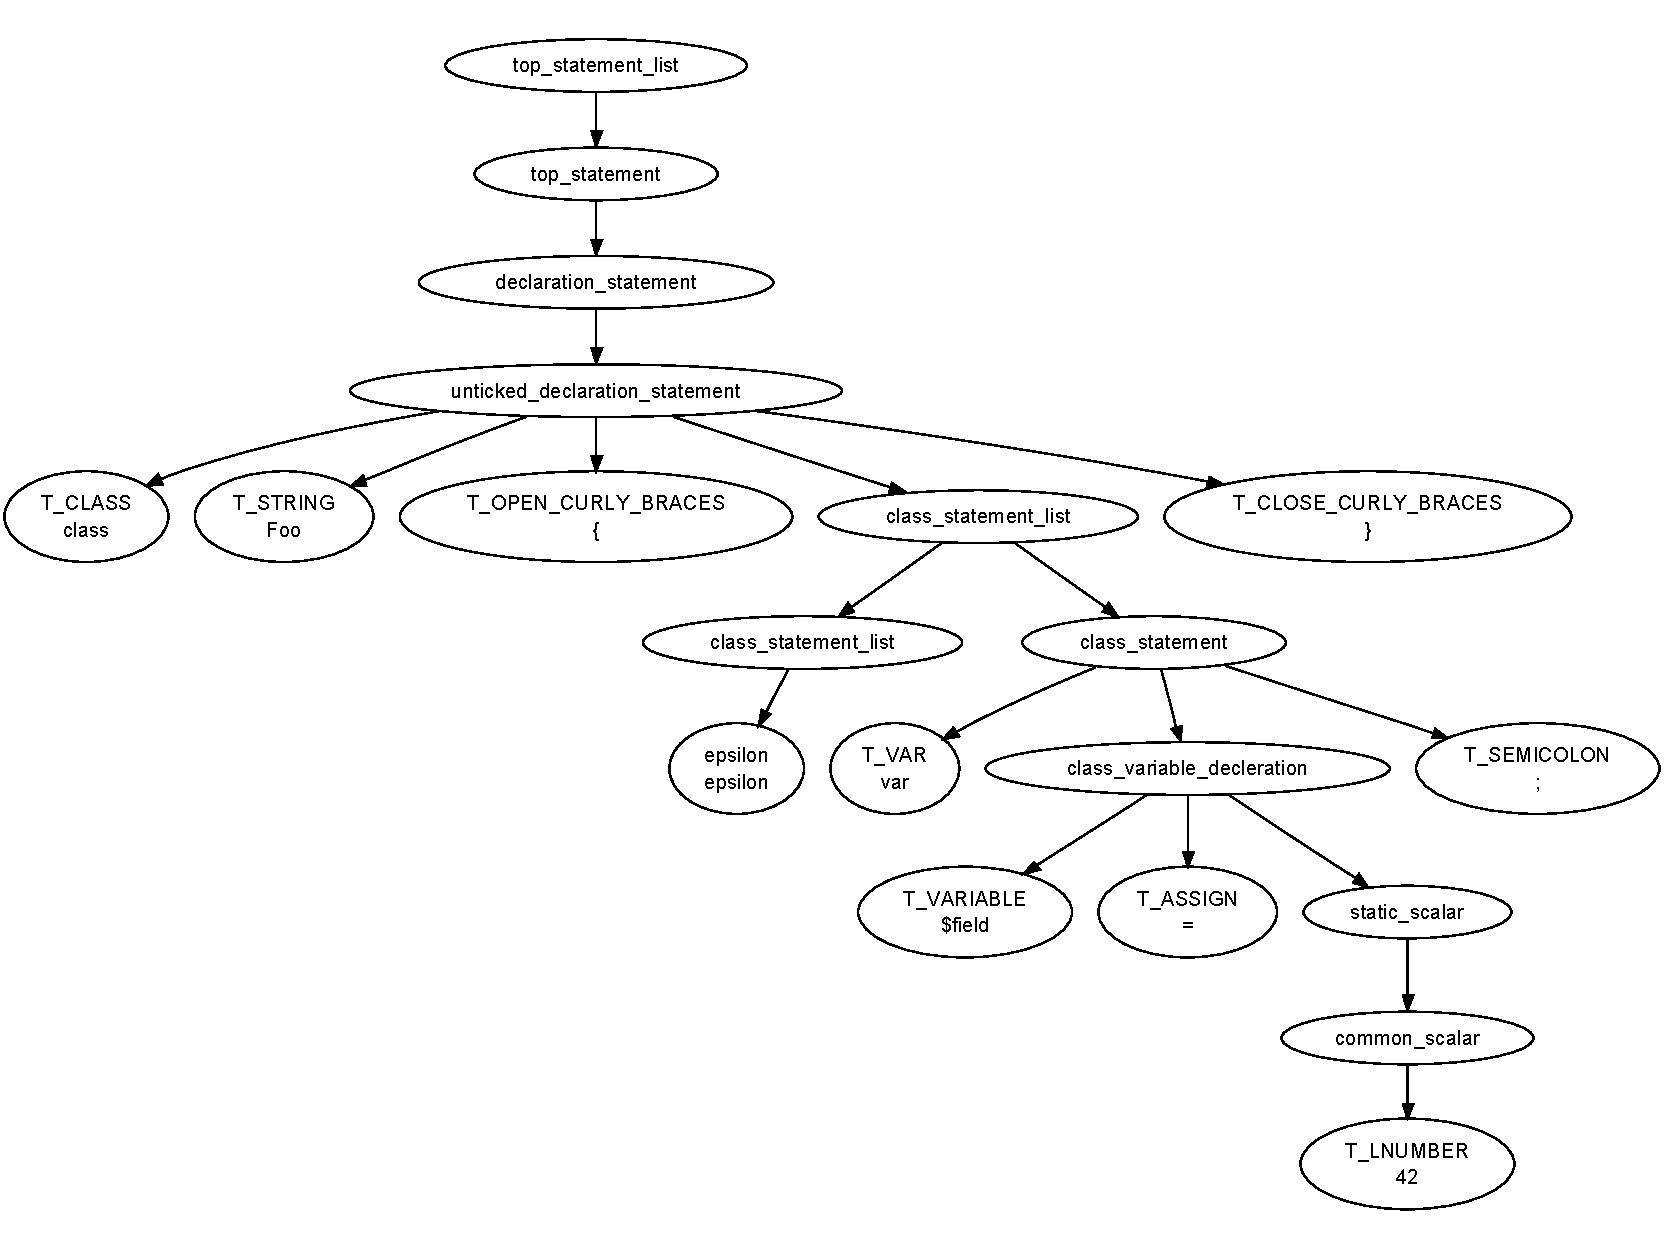
\includegraphics[width=\linewidth, height=.9\textheight, keepaspectratio]{images/parsetree-foo-class-declaration}
    \caption{The subtree of the PHP parse tree for declaring a class \texttt{Foo} with a single field \texttt{\$field} that has a default value of \texttt{42}.}
    \label{fig:parse-tree-foo-class}
  \end{center}
\end{figure}

At the point where Pixy's \texttt{TacConverter}\index{TacConverter} (section~\ref{tacconverter} on page~\pageref{tacconverter}) class encounters the class definition, it would be neither necessary nor helpful to save the taint state (section~\ref{taint-state} on page~\pageref{taint-state})\label{fields-not-saved-on-new} of the fields for new class instances: Member variables that have not been written yet by any code can always be considered untainted as the PHP interpreter only allows literals as default values, and Pixy always assumes literals to be untainted. Furthermore, uninitialized member variables cannot be overwritten using request parameters even if \texttt{register\_globals}\index{register\_globals} is enabled. This is different to the way PHP handles uninitialized local or global variables (see section~\ref{register-globals} on page~\pageref{register-globals}).

In addition, the list of declared fields might be a mere subset of the fields that are actually accessed in the code: If the PHP interpreter finds a read or write access to an undeclared field\index{undeclared fields}, it creates this field for that particular instance on the fly, initializes it with \texttt{null}, and issues a PHP strict warning.



\subsection{Storing Objects with Member Variables as Places for Three-Address Code (TAC)}
\index{member variables}\index{fields}\index{three-address code}

Pixy models variables as ``places''\index{place} for three-address code (see section~\ref{tac} on page~\pageref{tac} for details). The corresponding classes is named \texttt{AbstractPlace}\index{AbstractPlace}. For taint analysis, it uses this \emph{place} abstraction---instead of the variable directly from the parse tree---to model the flow of data through the program.

Hence, we need a way to convert access to member variables from the PHP parse tree into TAC places. This needs to happen within the \texttt{TacConverter}\index{TacConverter} class which is responsible for the task of creating both the control-flow graph as well as the three-address code from the PHP parse tree.

The \texttt{TacConverter} already adds a \texttt{Variable} entry into the current function's symbol table. To closely model the way PHP stores object instances with a separate symbol table per instance (see section~\ref{php-variables} on page~\pageref{php-variables}~ff.), we need a subclass \texttt{ObjectVariable extends Object}\index{ObjectVariable} that holds a reference to a symbol table instance---which then holds references to several \texttt{AbstractPlace} instances that represent the member variables.


\subsection{Field Access}

To track tainting for member variables, Pixy needs to create \emph{places} for all member variables that are accessed---even for those that have not been declared beforehand. (PHP will however happily create it on the fly while issuing a PHP warning.)

Both for the left side of assignments as well as for all expressions, we need to add a way to handle field access as places. In addition to the already existing cases (\eg function calls, literals, normal variables etc.), the following cases are new and need to be modeled:

\myTable{
\begin{tabular}{|l|l|l|}
\hline
\bb{case description} & \bb{example} & \bb{parse tree figure} \\
\hline
  simple variable assignment & \texttt{\$x = 42;}  & \ref{fig:simple-variable-assignment} on page~\pageref{fig:simple-variable-assignment} \\
  (already part of Pixy) & & \\
\hline
  one-level field access (left side) & \texttt{\$foo->bar = 42;} & \ref{fig:one-level-field-access-left} on page~\pageref{fig:one-level-field-access-left} \\
\hline
  one-level field access (right side) & \texttt{\$x = \$foo->bar;} & \ref{fig:one-level-field-access-right} on page~\pageref{fig:one-level-field-access-right} \\
\hline
  multi-level field access (left side) & \texttt{\$foo->bar->baz = 42;} & \ref{fig:multi-level-field-access-left} on page~\pageref{fig:multi-level-field-access-left} \\
\hline
  multi-level field access (right side) & \texttt{\$x = \$foo->bar->baz;} & \ref{fig:multi-level-field-access-right} on page~\pageref{fig:multi-level-field-access-right} \\
\hline
  variable field access (left side) & \texttt{\$foo->\$fieldName = 42;} & \ref{fig:variable-field-access-left} on page~\pageref{fig:variable-field-access-left} \\
\hline
  variable field access (right side) & \texttt{\$x = \$foo->\$fieldName;} & \ref{fig:variable-field-access-right} on page~\pageref{fig:variable-field-access-right} \\
\hline
\end{tabular}
}{Field accesses that need to be modeled}{table:field-access-cases}

\paragraph{Note:} Method chaining\index{method chaining} in PHP is possible, as is field access chaining\index{field access chaining}. After field chaining, method calls are possible. However, even if a method returns an object, chained field accesses on that object are not possible. This approach does not cover method call after field accesses as Pixy already is quite versed at finding out which method from which class gets called.


\begin{figure}[htb]
  \begin{center}
    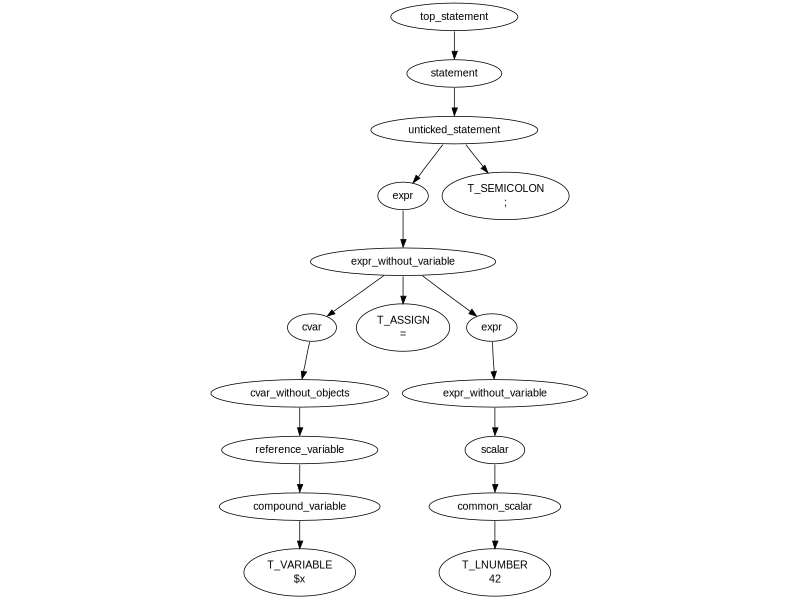
\includegraphics[scale=.7, trim=30mm 0mm 0mm 0mm]{images/simple-variable-assignment}
    \caption{The PHP parse subtree of \texttt{\$x = 42;}}
    \label{fig:simple-variable-assignment}
  \end{center}
\end{figure}

\begin{figure}[htb]
  \begin{center}
    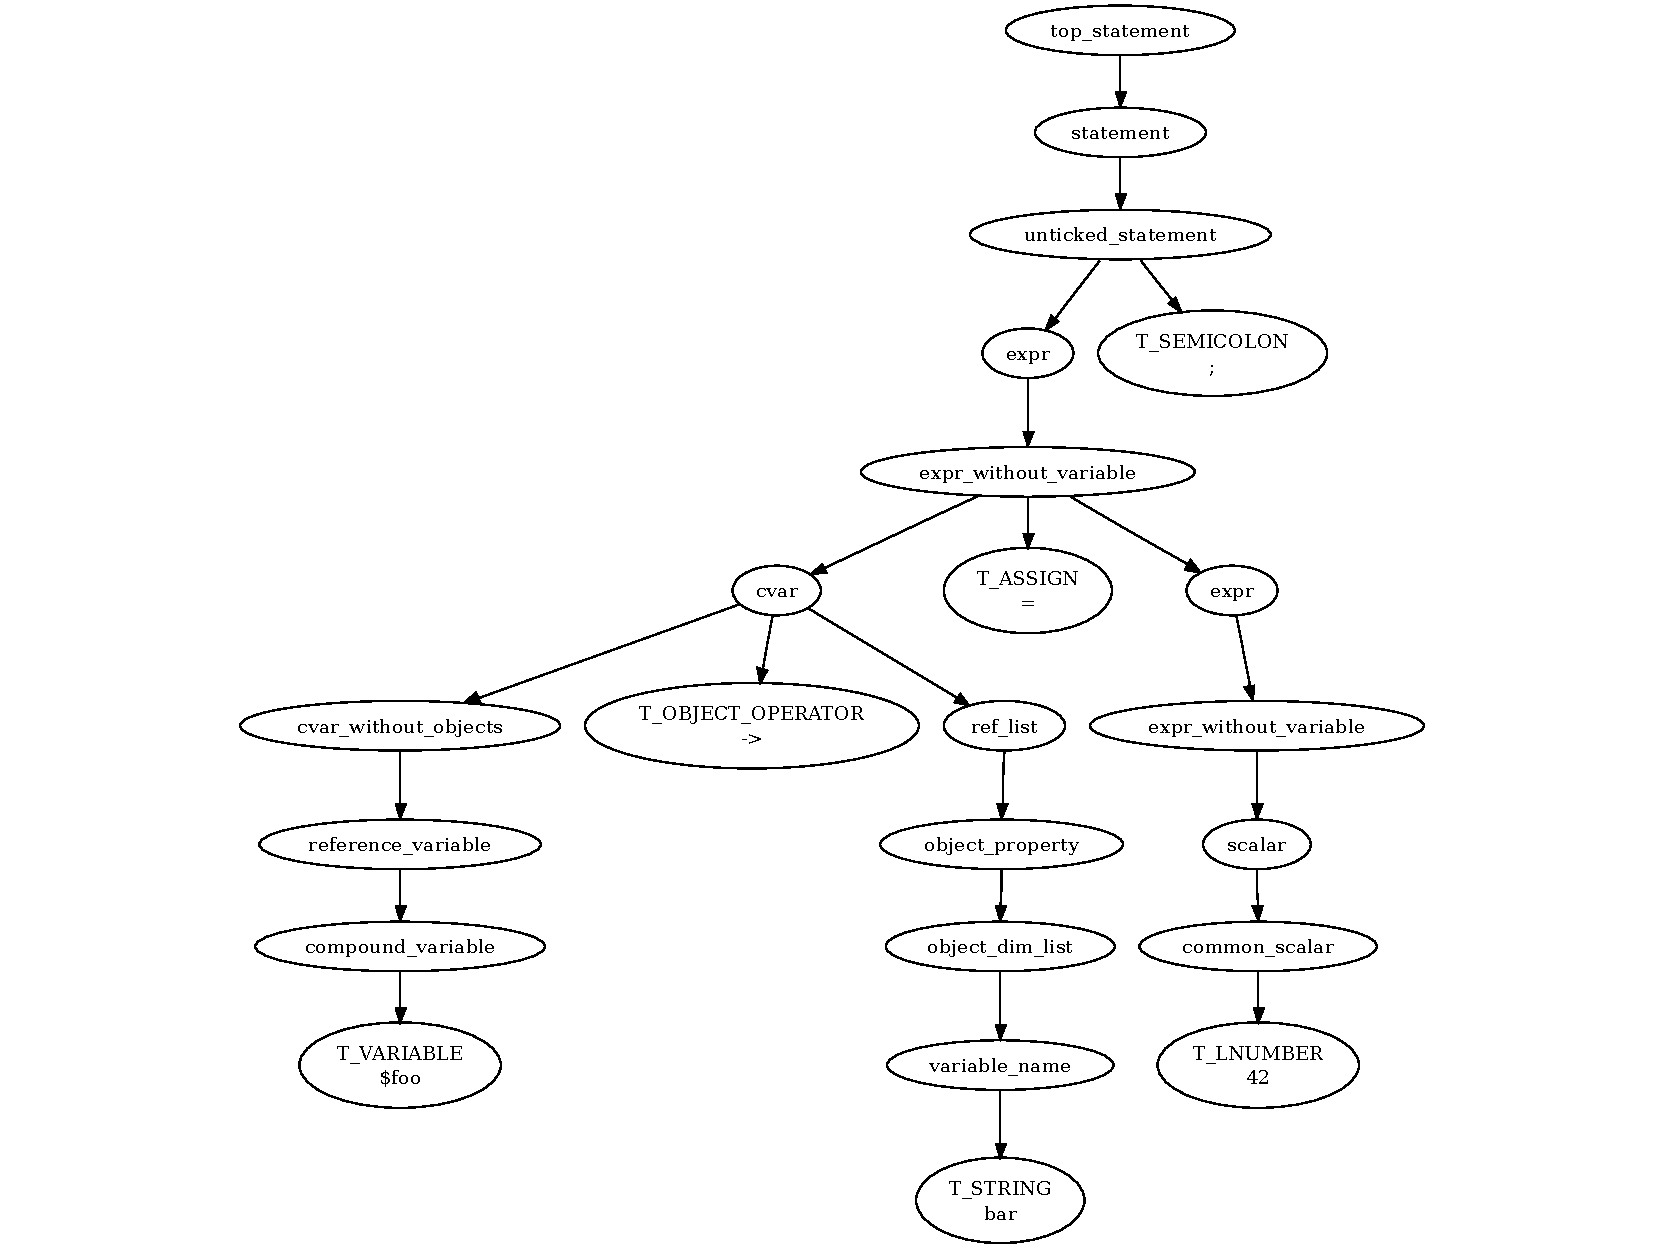
\includegraphics[scale=.73, trim=40mm 0mm 0mm 0mm]{images/one-level-field-access-left}
    \caption{The PHP parse subtree of \texttt{\$foo->bar = 42;}}
    \label{fig:one-level-field-access-left}
  \end{center}
\end{figure}

\begin{figure}[htb]
  \begin{center}
    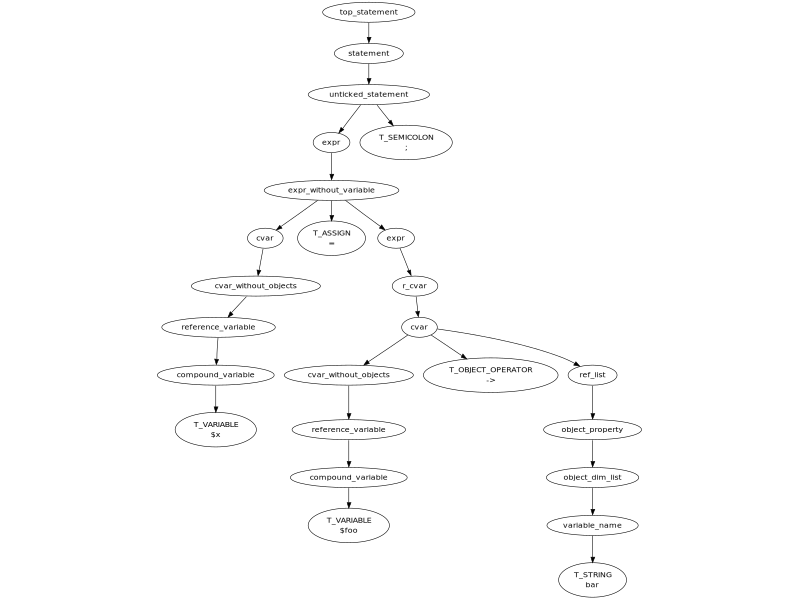
\includegraphics[scale=.85, trim=55mm 0mm 0mm 0mm]{images/one-level-field-access-right}
    \caption{The PHP parse subtree of \texttt{\$x = \$foo->bar;}}
    \label{fig:one-level-field-access-right}
  \end{center}
\end{figure}

\begin{figure}[htb]
  \begin{center}
    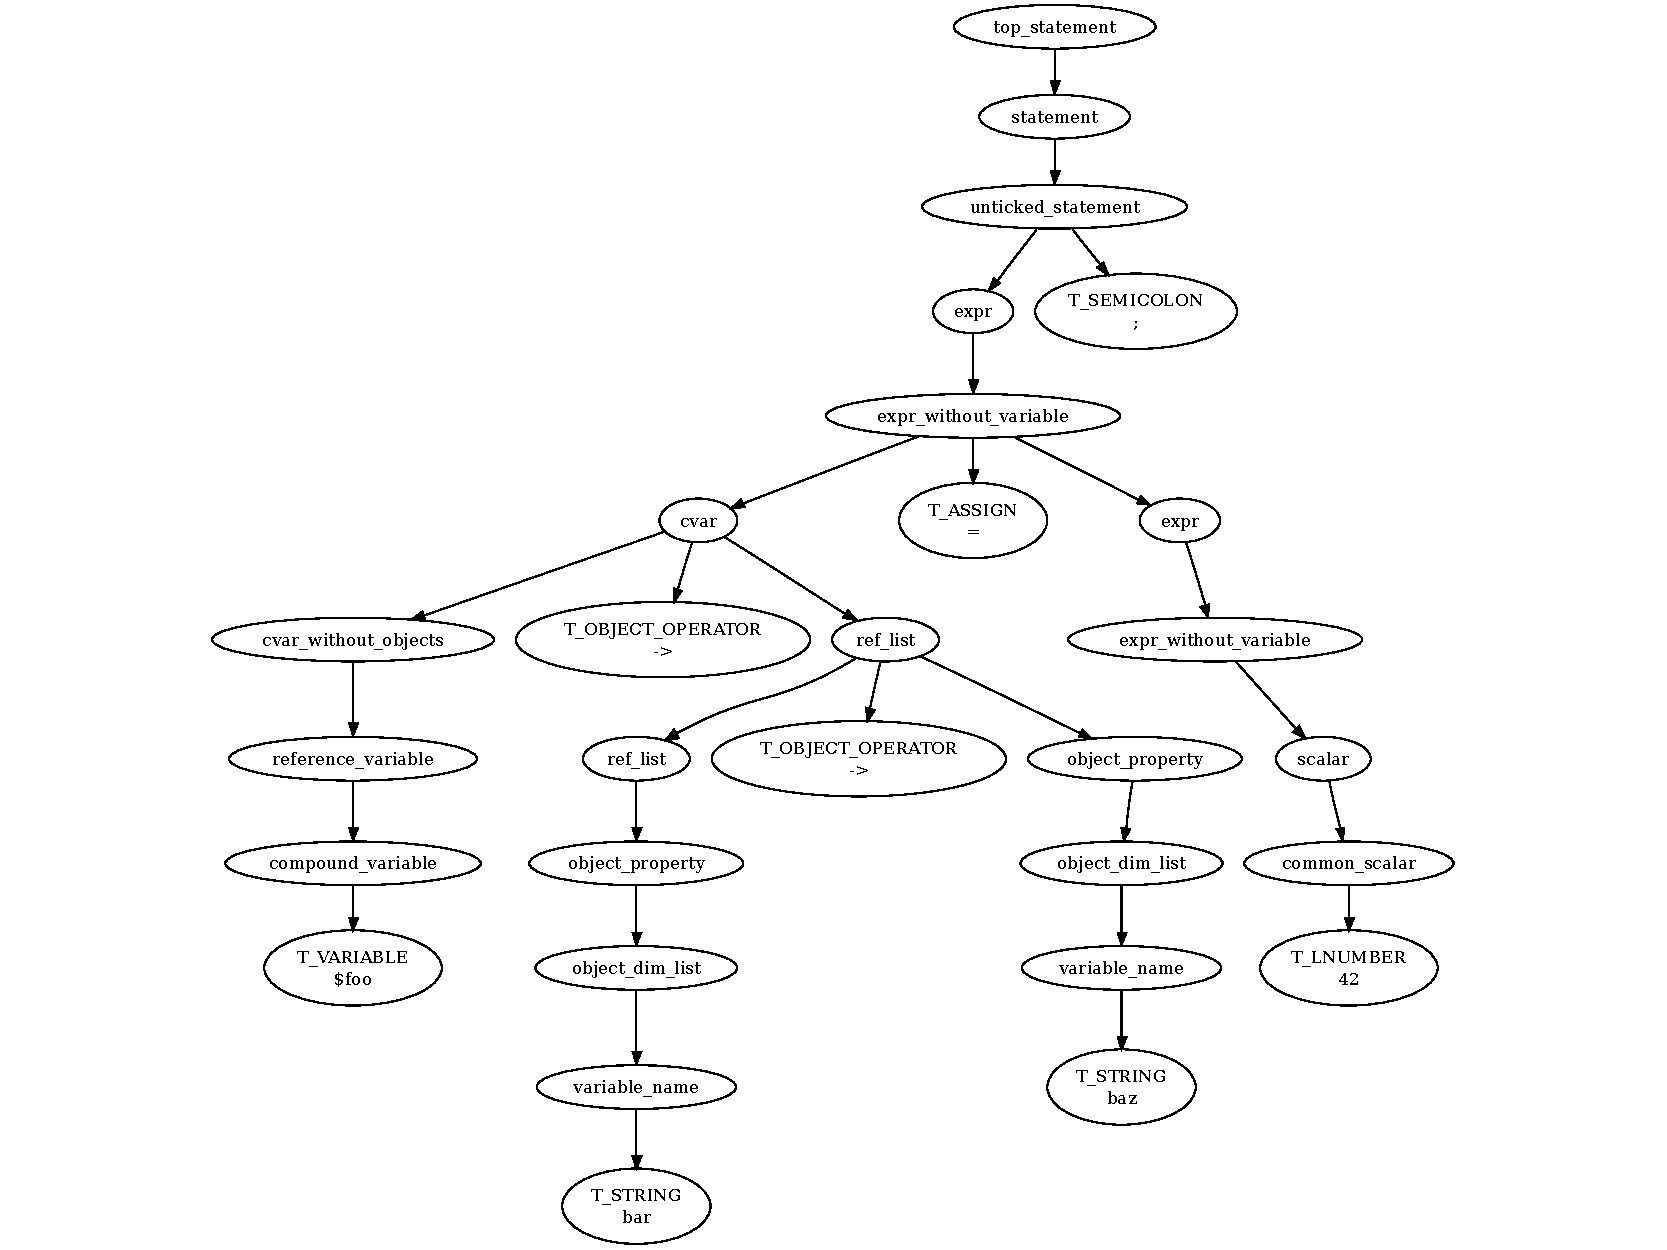
\includegraphics[scale=.7, trim=35mm 0mm 0mm 0mm]{images/multi-level-field-access-left}
    \caption{The PHP parse subtree of \texttt{\$foo->bar->baz = 42;}}
    \label{fig:multi-level-field-access-left}
  \end{center}
\end{figure}

\begin{figure}[htb]
  \begin{center}
    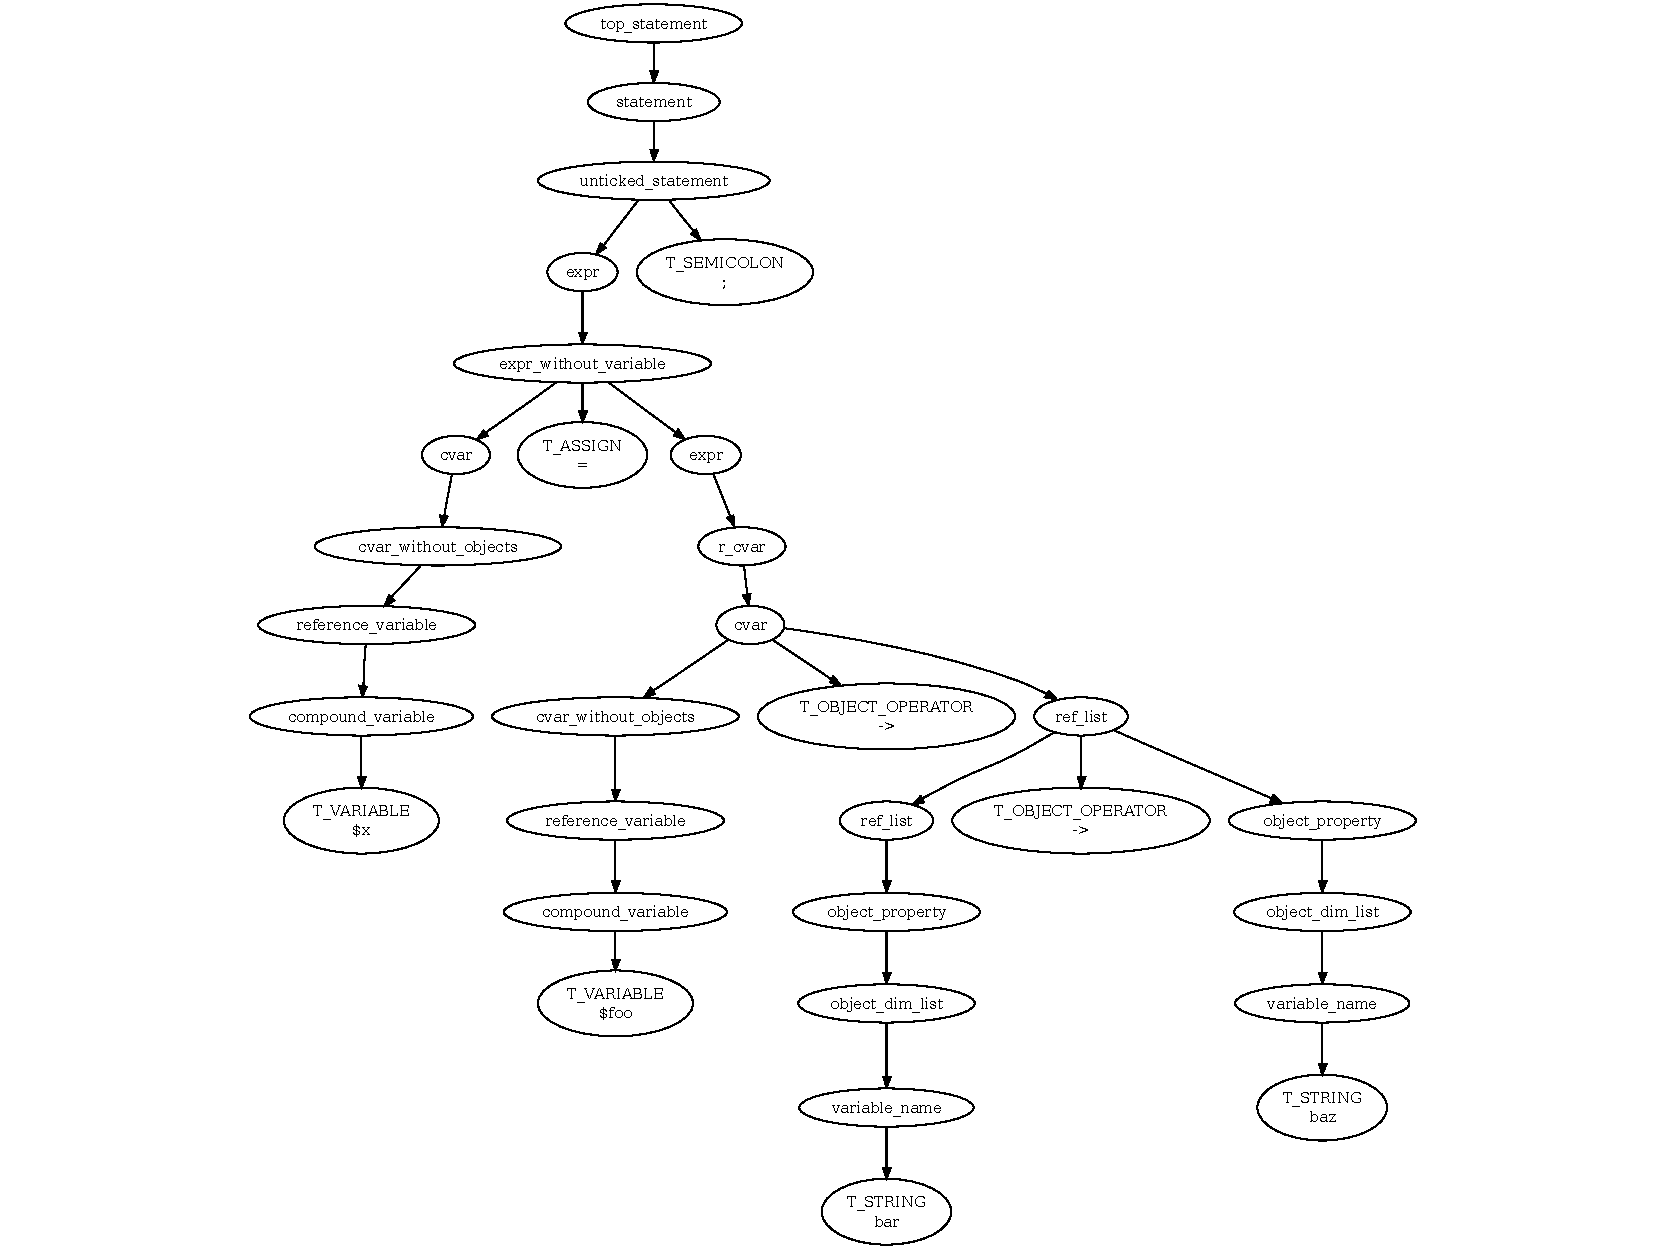
\includegraphics[scale=.74, trim=42mm 0mm 0mm 0mm]{images/multi-level-field-access-right}
    \caption{The PHP parse subtree of \texttt{\$x = \$foo->bar->baz;}}
    \label{fig:multi-level-field-access-right}
  \end{center}
\end{figure}

\begin{figure}[htb]
  \begin{center}
    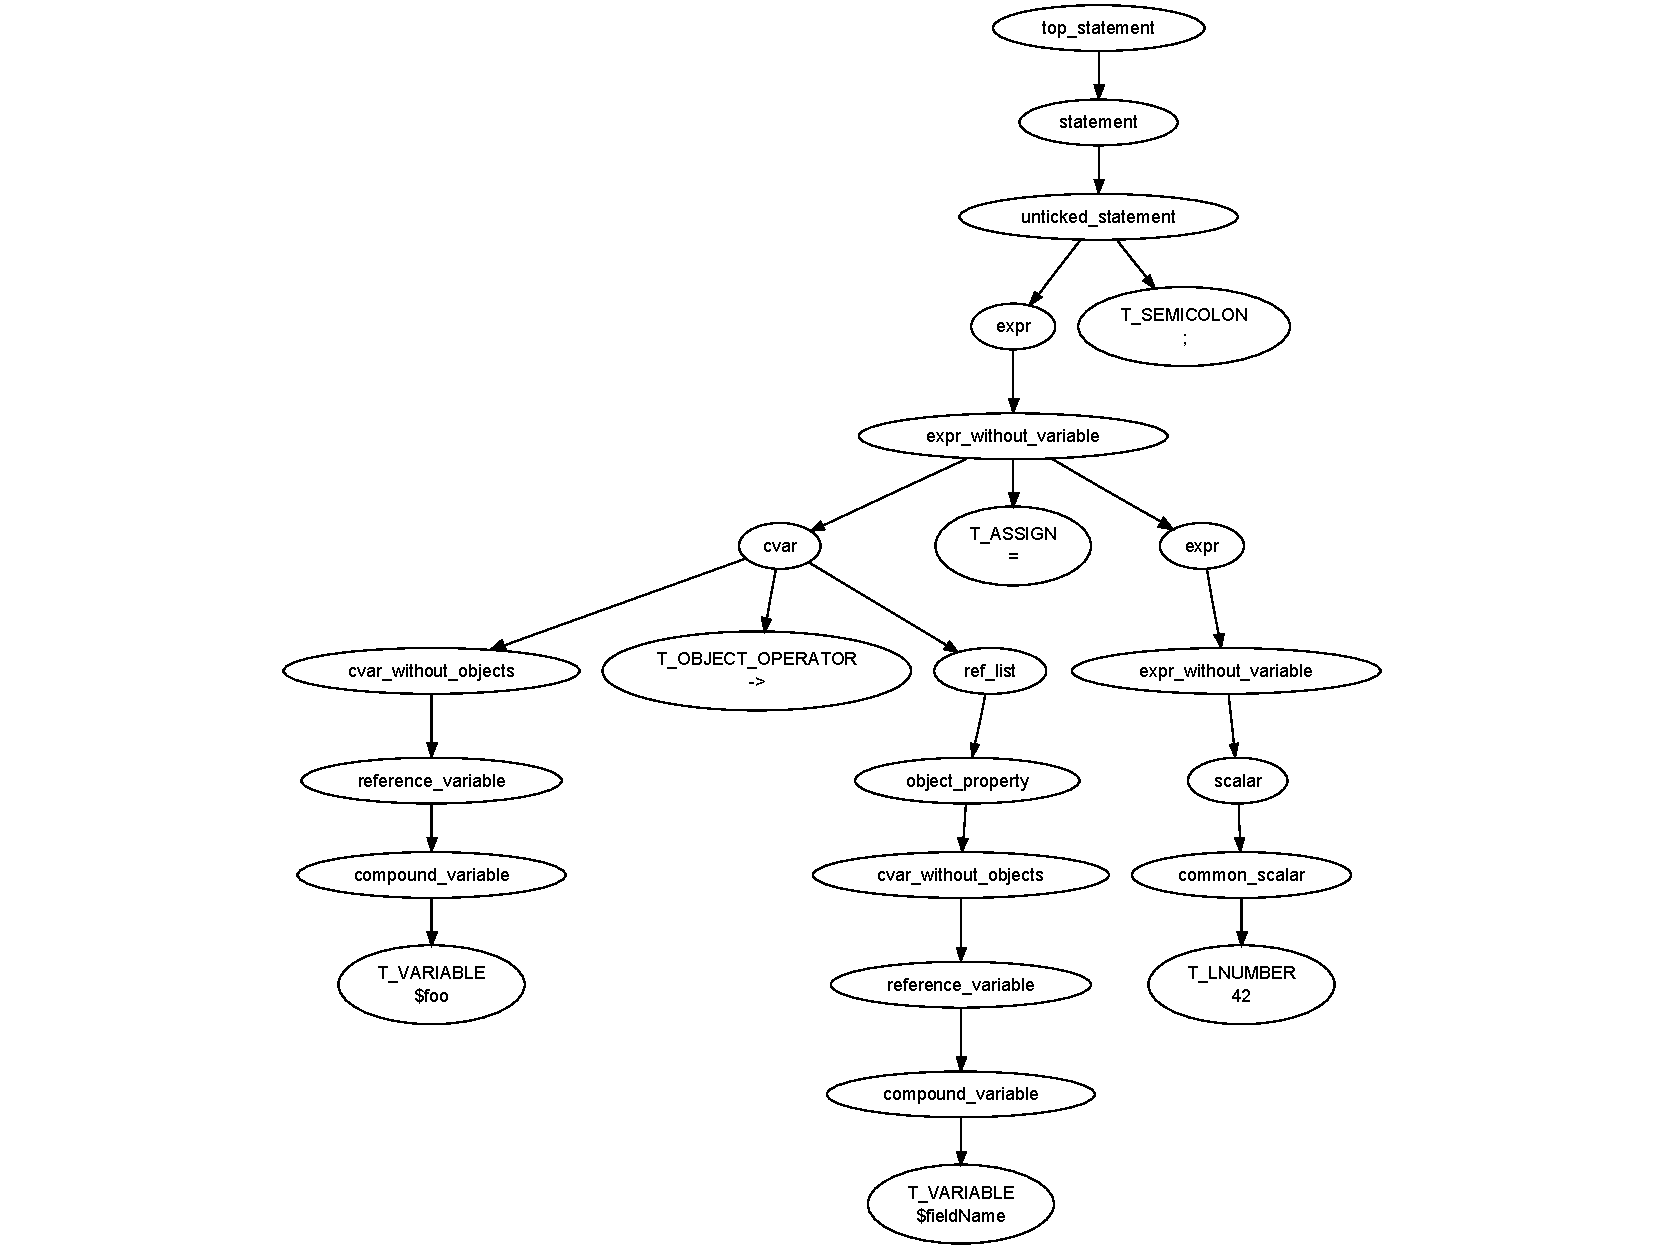
\includegraphics[scale=.78, trim=46mm 0mm 0mm 0mm]{images/variable-field-access-left}
    \caption{The PHP parse subtree of \texttt{\$foo->\$fieldName = 42;}}
    \label{fig:variable-field-access-left}
  \end{center}
\end{figure}

\begin{figure}[htb]
  \begin{center}
    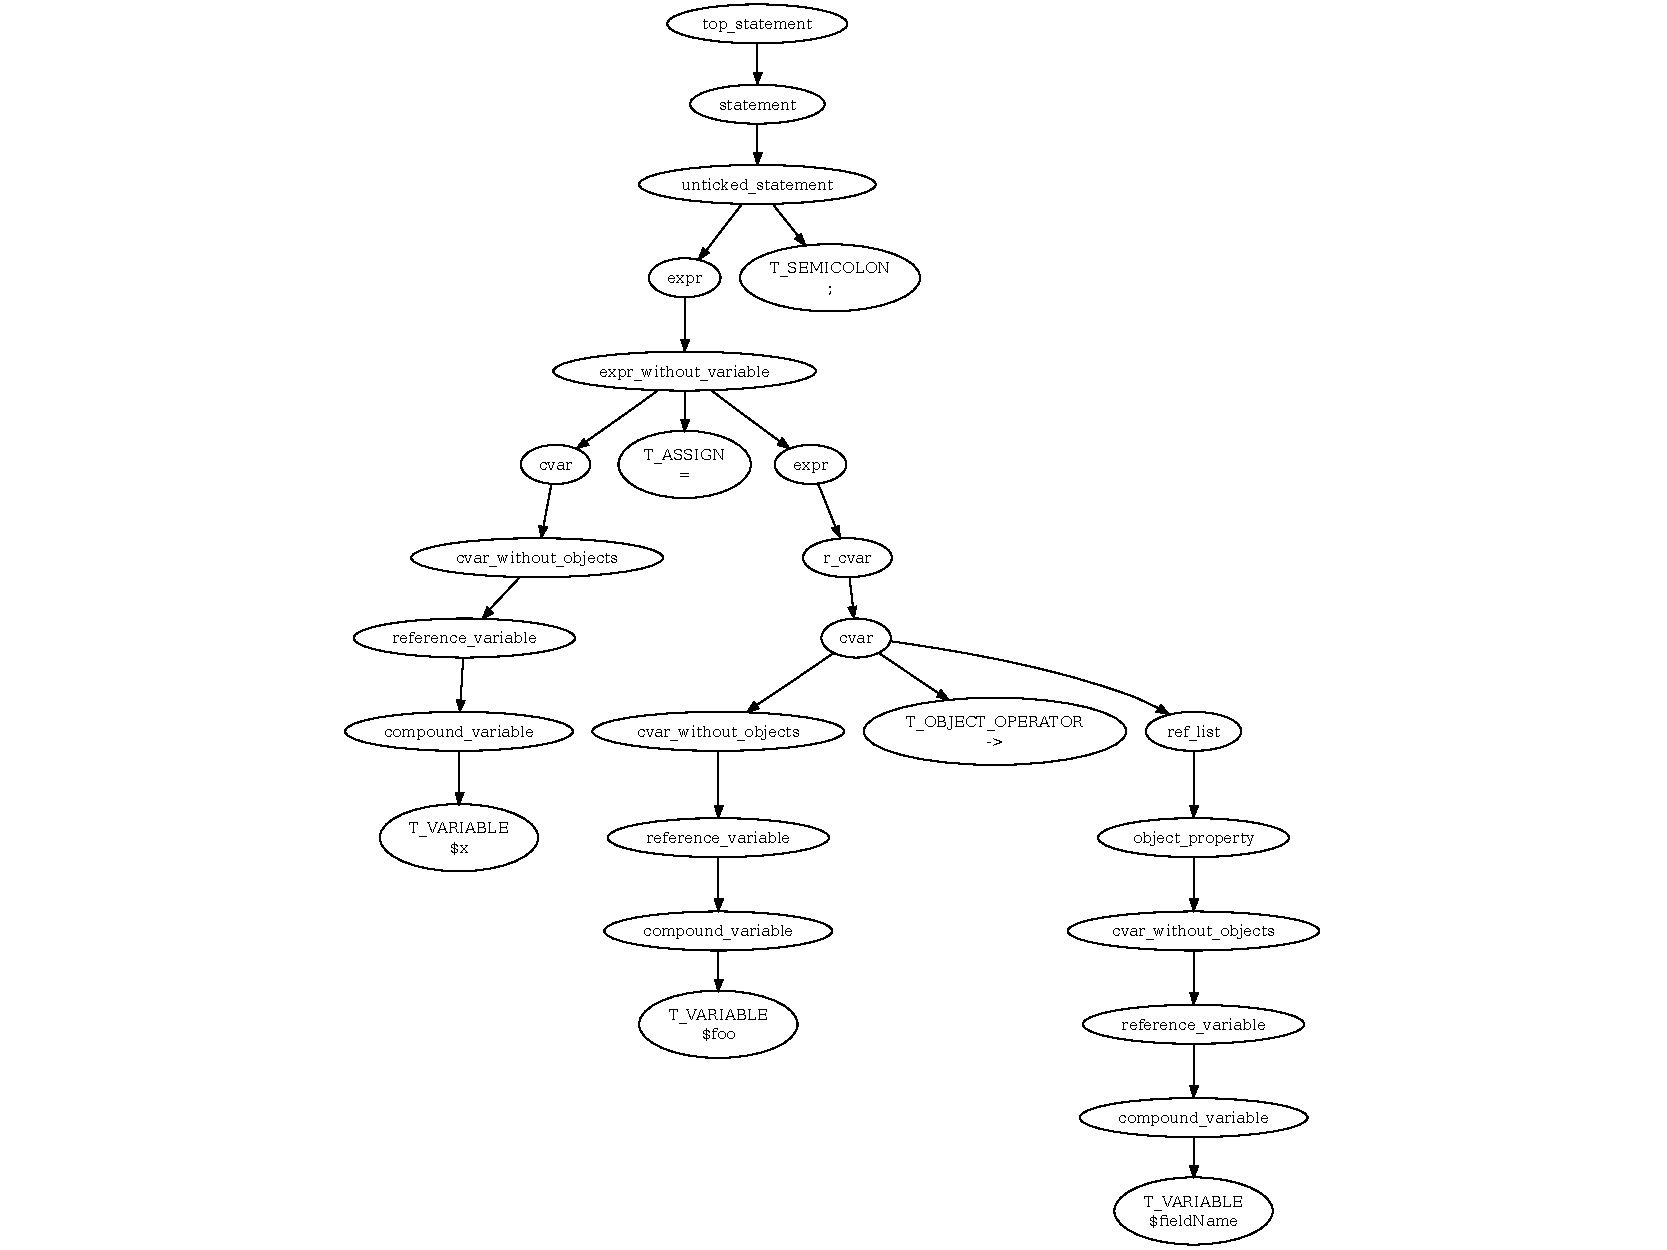
\includegraphics[scale=.9, trim=60mm 0mm 0mm 0mm]{images/variable-field-access-right}
    \caption{The PHP parse subtree of \texttt{\$x = \$foo->\$fieldName;}}
    \label{fig:variable-field-access-right}
  \end{center}
\end{figure}

As Pixy currently does not model the---relatively rare---case of variable variables\index{variable variables}, this approach does not model them on the field level either. Instead, this approach uses Pixy's special place \emph{specialPlaceForVariableVariables}\index{specialPlaceForVariableVariables} that keeps this place out of taint analysis.

Looking at the big picture, both for left-side\index{left-side expressions} and right-side expressions\index{right-side expressions}, the \texttt{TacConverter} walks the field access chain to the end, using existing fields in the object's symbol tables or creating new ones as required. There are two basic cases we need to cover: a write access to a place, \ie an assignment, and a read access---be it as the right part of an assignment, as part of a compound expression or as a parameter in a function call. In each and every case, the parse tree for the variable expression has a \texttt{cvar}\index{cvar} node in it. In other words: A \texttt{cvar} node in the parse tree is equivalent to a variable being accessed, \eg \texttt{\$a} or \texttt{\$foo->bar}.

This approach expands the \texttt{cvar} function to also return places for field accesses.

\paragraph{Note:} The listed pseudo-code takes a few shortcuts: It assumes that there are some convenience functions available for tree walking, array processing and string processing, and that functions like \texttt{cvar} return \texttt{AbstractPlace} instead of a \texttt{TacAttributes} wrapper.

\begin{javacode}
/**
 * Returns the AbstractPlace that corresponds to a cvar node in the
 * parse tree.
 */
AbstractPlace cvar(
  ParseNode subtreeRoot, SymbolTable functionSymbolTable
) {
  String[] nameChain = flattenCvarTreeToNameChain(subtreeRoot);

  return getLeftPlaceForNameChain(nameChain, functionSymbolTable);
}
\end{javacode}

\begin{javacode}
/**
 * Walks a cvar parse node subtree and extracts the variable name
 * or chained field names from it. The dollar sign from the first
 * variable is omitted.
 *
 * For example, for a variable foo, this function returns:
 * ["foo"]
 *
 * For a variable foo->bar->$baz, this function returns:
 * ["foo", "bar", "$baz"]
 */
String[] flattenCvarTreeToNameChain(ParseNode subtreeRoot) {
  String[] nameChain;

  for (ParseNode node : subTreeRoot.depthFirstIterator()) {
    Token token = node.token;
    if (!(token != T_VARIABLE && token != T_STRING) {
      continue;
    }

    // Drop the first dollar sign.
    if (nameChain.length == 0) {
      nameChain.append(node.text.dropFirstCharacter);
    } else {
      nameChain.append(node.text);
    }
  }

  return nameChain;
}
\end{javacode}

\begin{javacode}
/**
 * Gets the AbstractPlace for a variable name chain from symbolTable.
 *
 * If there is no place with that name yet, it will be created on the
 * fly (if possible).
 */
AbstractPlace getLeftPlaceForNameChain(
  String[] nameChain, SymbolTable symbolTable
) {
  String firstElementInNameChain = nameChain[0];
  if (isVariableVariable(firstElementInNameChain)) {
    return specialPlaceForVariableVariables;
  }

  if (nameChain.length == 1) {
    return getOrCreateVariableInSymbolTable(
      firstElementInNameChain. symbolTable
    );
  }

  // At this point, we have more than one element in the name chain,
  // i.e., a field access.
  if (!symbolTable.has(firstElementInNameChain)) {
    throw new Exception("Field access on nonexistent object.");
  }

  AbstractPlace firstPlaceFromNameChain = symbolTable.getByName(
    firstElementInNameChain
  );
  if (!firstPlaceFromNameChain instanceof ObjectVariable) {
    throw new Exception("Field access on non-object variable.");
  }

  String[] nameChainWithoutFirstElement = nameChain.dropFirst();
  return getLeftPlaceForNameChain(
    nameChainWithoutFirstElement,
    ((ObjectVariable) firstPlaceFromNameChain).symbolTable
  );
}
\end{javacode}

\begin{javacode}
/**
 * Retrieves the Variable stored under the given variableName from
 * the symbolTable.
 *
 * If there is no entry for that variableName yet, creates a new
 * Variable entry, stores it in the symbolTable and returns it.
 */
Variable getOrCreateVariableInSymbolTable(
  String variableName, SymbolTable symbolTable
) {
  if (symbolTable.has(variableName)) {
    return symbolTable.getByName(variableName))
  }

  Variable newVariable = new Variable();
  symbolTable.addByName(variableName, newVariable);

  return newVariable;
}
\end{javacode}


\subsection{Class Instantiation}

When a class gets instantiated, the \texttt{TacConverter} needs to create a symbol table entry to store a new \texttt{ObjectVariable}\index{ObjectVariable} instance in.

In the following code example, the \texttt{Foo} class declared above gets instantiated in the \texttt{\$foo} variable. The corresponding subtree of the PHP parse tree looks like figure~\ref{fig:parse-tree-new-foo} on page~\pageref{fig:parse-tree-new-foo}.

\begin{phpcode}
$foo = new Foo();
\end{phpcode}

\begin{figure}[htb]
  \begin{center}
    \includegraphics[width=\linewidth, height=.9\textheight, keepaspectratio]{images/parsetree-new-foo}
    \caption{The subtree of the PHP parse tree for creating an instance \texttt{\$foo} of the class \texttt{Foo}.}
    \label{fig:parse-tree-new-foo}
  \end{center}
\end{figure}

In pseudo-code, processing this assignment would look like this:\index{expr\_without\_variable}

\begin{javacode}
/**
 * Processes an expr_without_variable node and returns the
 * AbstractPlace contained in the node (if any).
 */
AbstractPlace expr_without_variable(ParseNode subtreeRoot) {
  if (subtreeRoot.secondChild() == T_ASSIGN) {
    // We take for granted that TacConverter already has an assign()#
    // function.
    assign(subtreeRoot);
    return null;
  }

  if (firstChild == T_NEW) {
    return new ObjectVariable();
  }

  // More existing code for processing variables and literals.
}
\end{javacode}

\paragraph{Note:} In the \texttt{TacConverter} class, the functions are named after the opcodes in the PHP parse tree. The function \texttt{expr\_without\_variable} is called twice because it occurs twice in the subtree (see figure~\ref{fig:parse-tree-new-foo} on page~\pageref{fig:parse-tree-new-foo}).

For the sake of brevity, this pseudo-code omits the part about creating temporary variables if a variable already is present in the symbol table. This feature already exists in Pixy and does not need to be changed.


\section{Alias Analysis for Objects and Fields}

An alias analysis for objects needs to take two aspects into account: that objects are passed by reference (see section~\ref{object-references} on page~\pageref{object-references}), and the alias relationships between fields. This is an important aspect because objects cannot have a taint status, while their fields can.


\subsection{Object References}
\index{object references}

In addition to the must-aliases and may-aliases, Pixy needs to track references between objects. In order to do so, Pixy needs to leverage its existing type detection for variables. The approach to object references is quite similar to that for variables aliases: As with may-aliases and must-aliases for variables, the analysis tracks \emph{must-references}\index{must-reference}\index{reference!must \see{must-reference}} and \emph{may-references}\index{may-reference}\index{reference!may \see{may-reference}} for objects.

In the object reference analysis, the same cases are relevant as with the alias analysis: assignments, \texttt{unset} calls, and function calls with parameters.


\subsubsection{Assignments}

Let's assume that there are no must-references and may-references yet:

$mustReferences = \{\}, mayReferences = \{\}$

If an object is created and then copied to another variable, the pair of both variables is added to the $mustReferences$ set:

\begin{phpcode}
$foo = new Foo();
$bar = $foo;
\end{phpcode}

$mustReferences = \{(foo, bar)\}, mayReferences = \{\}$

If there is a condition, the must-reference is changed to a may-reference after the end of the condition:

\begin{phpcode}
$foo = new Foo();

if (...) {
  $bar = $foo;
}
\end{phpcode}

$mustReferences = \{\}, mayReferences = \{(foo, bar)\}$

If an existing variable that is listed in the must-references or may-references is overwritten, it needs to get removed from the references:

$mustReferences = \{\}, mayReferences = \{(foo, bar)\}$

\begin{phpcode}
$bar = 42;
\end{phpcode}

$mustReferences = \{\}, mayReferences = \{\}$

All of these steps can be repeated with several commands, causing the reference sets to change accordingly. For example, a variable can first be used for a reference and then be overwritten with a different reference, causing the first reference to be deleted and the new reference to be created:

\begin{phpcode}
$foo = new Foo();
$bar = $foo;

$foo2 = new Foo();
$bar = $foo2;
\end{phpcode}

$mustReferences = \{(bar, foo2)\}, mayReferences = \{\}$

If a must-reference is overwritten during a condition, it gets changed to a may-reference, and the new reference is added as a may-reference just as in the example above:

\begin{phpcode}
$foo = new Foo();
$bar = $foo;

$foo2 = new Foo();
if (...) {
  $bar = $foo2;
}
\end{phpcode}

$mustReferences = \{\}, mayReferences = \{(bar, foo), (bar, foo2)\}$

\paragraph{Note:} This only affects assignments by value. Assignments by reference (using the \texttt{=~\&} assigment operator) still are real aliases and are handled accordingly.\index{assigning by reference}


\subsubsection{Unset Calls}
\index{unset}

An \texttt{unset} call removes the corresponding object variable from all must-references and may-references:

$mustReferences = \{(bar, foo)\}, mayReferences = \{(bar, foo2)\}$

\begin{phpcode}
unset($bar);
\end{phpcode}

$mustReferences = \{\}, mayReferences = \{\}$


\subsubsection{Function Calls}
\index{function calls}

As function parameters are passed by value---which in the case of objects means a copy of object handle pointing to one and the same object---, this creates a reference from the caller's object variable and the callee's parameter.

$mustReferences = \{\}, mayReferences = \{\}$

\begin{phpcode}
function someFunction() {
  $foo = new Foo();
  otherFunction(foo);
}

function otherFunction(Foo $foo) {
\end{phpcode}

At this point within the \texttt{otherFunction} function, there is a must-reference:

$mustReferences = \{(someFunction.foo, otherFunction.foo)\}, mayReferences = \{\}$

\paragraph{Note:} The dot notation for the function name in the variable names within the reference sets is the same as in the alias sets used in section~\ref{sec:aliases-globals} on page~\pageref{sec:aliases-globals}.


\subsection{Field Aliases}
\index{field alias}\index{member variable alias \see{field alias}}

As mentioned further above in section~\ref{fields-not-saved-on-new}, it is not helpful to store the fields of an object at the point of instantiation as far as tainting is concerned. Instead, the fields need to be added on the fly as they are read or written.


\subsubsection{Field Accesses}
\index{field accesses}

When a field is written or read, the alias analyzer needs to check and update alias information for that field and then take the corresponding line of code into further alias analysis. After a field has been added as a must-alias or may-alias, Pixy's existing alias analysis can kick in.

The basic rules at that point are:

\begin{itemize}
  \item Create field must-aliases for all must-aliases and must-references of the particular object.
  \item Create field may-aliases for all may-aliases and may-references of the particular object.
\end{itemize}


\paragraph{Object aliases}
\index{object alias}

Let's have a look at an example for object aliases first. At the beginning, we already have one must-alias and one may-alias for some objects:

$mustAliases = \{(a, b)\}, mayAliases = \{(a, c)\}$

Now a field is accessed, causing the field to be created if it does not exist at that point:

\begin{phpcode}
$x = $a->name;
\end{phpcode}

Before any further alias information for this line of code is evaluated, the alias information gets updated as follows:

$mustAliases = \{(a, b), (a.name, b.name)\}, mayAliases = \{(a, c), (a.name, c.name)\}$


\paragraph{Object references}
\index{object references}

A similar example with object references instead of object aliases works basically the same:

$\begin{array}{llll}
mustReferences & = \{(a, b)\}, & mayReferences & = \{(a, c)\} \\
mustAliases & = \{\}, & mayAliases & = \{\}
\end{array}$

\begin{phpcode}
$x = $a->name;
\end{phpcode}

$\begin{array}{llll}
mustReferences & = \{(a, b)\}, & mayReferences & = \{(a, c)\} \\
mustAliases & = \{(a.name, b.name)\}, & mayAliases & = \{(a.name, c.name)\}
\end{array}$


\subsubsection{Unset: Removing aliases or references}
\index{unset}

When an object variable is dropped from the symbol table via \texttt{unset}, all occurrences of this object's fields need to be removed from all must-aliases and may-aliases.

For example, we have the following must-aliases and may-aliases:

$\begin{array}{ll}
mustAliases & = \{(a, b), (x, y), (a.name, b.name), (x.name, y.name)\} \\
mayAliases & = \{(a, c), (x, z), (a.name, c.name), (x.name, z.name)\}
\end{array}$

Now \texttt{\$a} gets unset:

\begin{phpcode}
unset($a);
\end{phpcode}

After \texttt{\$a} has been unset, the pruned alias sets do not contain any fields of \texttt{\$a} anymore:

$\begin{array}{ll}
mustAliases & = \{(x, y), (x.name, y.name)\} \\
mayAliases & = \{(x, z), (x.name, z.name)\}
\end{array}$


\subsubsection{Changing Must-Aliases to May-Aliases}
\index{may-alias}

When a must-alias for an object is changed to a may-alias or a must-reference is changed to a may-reference, the field alias information need to be changed accordingly.

Let's say we are within a condition:

\begin{phpcode}
$a = new Foo();
if (...) {
  $b = $a;
  $b->name = $x;
\end{phpcode}

Still within the condition, \texttt{\$b} and \texttt{\$a} are must-references, and the fields correspondingly are must-aliases, too:

$\begin{array}{llll}
mustReferences & = \{(a, b)\}, & mayReferences & = \{\} \\
mustAliases & = \{(a.name, b.name)\}, & mayAliases & = \{\}
\end{array}$

After the end of the condition, the must-reference gets changed to a may-reference, and the must-aliases of the field get changed to may-aliases:

\begin{phpcode}
$a = new Foo();
if (...) {
  $b = $a;
  $b->name = $x;
}
\end{phpcode}

$\begin{array}{llll}
mustReferences & = \{\}, & mayReferences & = \{(a, b)\} \\
mustAliases & = \{\}, & mayAliases & = \{(a.name, b.name)\}
\end{array}$

